\documentclass[10pt,twoside,a4paper,UTF8]{ctexbook}

\usepackage{listings}
\usepackage{xcolor}
\usepackage{geometry} % 页面布局
\geometry{a4paper, margin=1in} % 设置纸张大小和边距
\usepackage{titlesec}
\usepackage{geometry}
\usepackage{amsmath}
\usepackage[hidelinks]{hyperref} %将目录加上链接,并取消红色方框
\usepackage{graphicx}
\usepackage{float}
\usepackage{amssymb}
\usepackage{amsmath}
\usepackage{fancyhdr}

\usepackage{xpatch}
\makeatletter
\xpatchcmd{\chapter}
{\cleardoublepage}{\clearpage}
{}{}
\makeatother

\pagestyle{fancy}
\fancyhf{}
\fancyhead[OR]{\rightmark \ \ \ \ \thepage}
\fancyhead[EL]{\thepage \ \ \ \ \leftmark}
\renewcommand{\chaptermark}[1]{\markboth{第 \thechapter 章\ #1}{}}
\renewcommand{\sectionmark}[1]{\markright{\thesection \ \ #1}}

\titleformat{\part}
{\heiti\Huge\centering}
{第 \thepart 部分}
{1em}{}

\titleformat{\chapter}
{\heiti\huge}
{第 \thechapter 章}
{1em}{}

\titleformat{\section}
{\heiti\Large}
{\thesection}
{1em}{}

\titleformat{\subsection}
{\heiti\large}
{\thesubsection}
{1em}{}

\titleformat{\subsubsection}
{\heiti}
{}
{0em}{}

\usepackage{xpatch}
\makeatletter
\xpatchcmd{\chapter}
{\cleardoublepage}{\clearpage}
{}{}
\xpatchcmd{\part}
{\cleardoublepage}{\clearpage}
{}{}
\makeatother

%设置代码块(这样好看)
\lstset
{
	numbers=left,
	language=C++,                                                                            % 语言
	frame=shadowbox,
	keywordstyle=\color{blue!70}\bfseries,                                 % 设置关键字为粗体,颜色为 blue!70
	commentstyle=\color{olive},                                                    % 设置注释样式
	rulesepcolor=\color{red!20!green!20!blue!20!},                   % 设置框架阴影颜色
	basicstyle=\small\ttfamily,                                                       % 设置字体簇
	stringstyle = \color{purple},                                                     % 字符串颜色
	showstringspaces = false,                                                        % 显示字符串中的空格
	breaklines=true,                                                                         % 自动换行
	columns=flexible,                                                                       % 紧凑一些
	numberstyle=\footnotesize,                                                     % 缩小行号
	frameround=tttt,                                                                        % 边框圆角
	tabsize=4,                                                                                     % 缩进空格数
}

\setmonofont{Consolas}
\setCJKmonofont{SimHei}

\title{编程学习笔记}
\author{Awsdkl}
\date{\today}
\begin{document}
	\maketitle
	\tableofcontents
%==============================================字符串=============================================
	\part{字符串}
	\chapter{字符串}
	\section{字符串匹配}
	字符串匹配又被称为模式匹配(pattern matching),简单来说就是在主串 $s$ 中寻找子串 $t$。而字符串 $t$ 被成为 \texttt{模式串}(pattern)。 \par
	\subsection{暴力做法}
	这种做法非常简单。思想主要就是从主串 $s$ 的第一个字符开始和模式串 $t$ 的第一个字符开始匹配,若相等,则比较二者后续的字符。若不匹配,则模式串 $t$ 退回到第一个字符,与主串 $s$ 的下一个字符比较。如此循环往复,直至 $s$ 与 $t$ 都比较完毕。\par
	不难发现这种算法的时间复杂度在最坏情况下为 $O(|s|\cdot|t|)$,是非常大的。
	\subsection{KMP 算法}
	
	\subsubsection{前缀函数}
	给定一个长度为 $m$ 的字符串 $t$,则其前缀数组 $nxt_i$ 表示:$t$ 的第 $1$ 至 $i$ 位中前缀和后缀相同的部分的长度。
	\subsubsection{代码}
	\begin{lstlisting}
char s[MAXN],t[MAXN];
int n,m;
int nxt[MAXN];

void init()
{
	for(int i = 2,j = 0;i <= m;i++)
	{
		while(j && t[i] != t[j+1]) j = nxt[j];
		if(t[i] == t[j+1]) j++;
		nxt[i] = j;
	}
}
	\end{lstlisting}
	\subsection{查找}
	\subsubsection{代码}
	\begin{lstlisting}
void Match()
{
    for(int i = 1,j = 0;i <= n;i++)
    {
        while(j && s[i] != t[j+1]) j = nxt[j];
        if(s[i] == t[j+1]) j++;
        if(j == m)
        {
            //找到了
        }
    }
}
	\end{lstlisting}
	\section{Lyndon 分解}
	我们首先介绍 Lyndon 分解的概念。
	
	Lyndon 串是指对于一个字符串 $s$,若 $s$ 的字典序严格小于 $s$ 的所有后缀的字典序,则称 $s$ 为 Lyndon 串。换句话说,当且仅当 $s$ 的字典序严格小于它的所有非平凡的循环同构串时,$s$ 为 Lyndon 串。
	
	Lyndon 分解指将串 $s$ 分解为 $s = w_1 w_2 \cdots w_k$,其中所有 $w_i$ 均为 Lyndon,且它们的字典序按照非严格单调递减排序。
	
	\subsection{Duval 算法}
	Duval 算法可以在 $O(n)$ 的时间复杂度内求出一个串的 Lyndon 分解。
	
	这里我们先引出近似 Lyndon 串的概念。如果一个字符串 $s$ 能被分解成 $s = ww\cdots\bar w$ 的形式,其中 $w$ 为 Lyndon 串,$\bar w$ 为 $w$ 的一个前缀(可能为空),则称 $s$ 为一个近似 Lyndon 串。同时,一个 Lyndon 串也是一个近似 Lyndon 串。
	
	Duval 算法用了贪心的思想。在算法过程中,我们将带分解串 $s$ 分成三个部分 $s=s_1s_2s_3$,其中 $s_1$ 是已经分解好的部分,$s_2$ 是一个近似 Lyndon 串,$s_3$ 是未处理部分。
	\subsubsection{过程}
	在算法中,我们会尝试将 $s_3$ 的首字符添加到 $s_2$ 的末尾,然后判断 $s_2$ 是否仍为近似 Lyndon 串。若不是,则我们将 $s_2$ 的前缀是 Lyndon 的部分接到 $s_1$ 的末尾。
	
	具体的,我们需要维护三个变量 $i, j, k$。其中,$i$ 指向 $s_2$ 的首字符,并从 $1$ 遍历到 $n$。$j$ 指向 $s_3$ 的首字符。$k$ 指向 $s_2$ 中我们当前考虑的字符,即 $j$ 在 $s_2$ 的上一个循环节中对应的字符。我们的目标是将 $s_j$ 加到 $s_2$ 的末尾,这就需要 $s_j$ 与 $s_k$ 做比较。
	
	不难推出三种比较的情况如下:
	\begin{itemize}
		\item $s_j = s_k$:将 $s_j$ 加到 $s_2$ 末尾并不会影响 $s_2$ 近似 Lyndon 串的性质。则将 $j, k$ 自增即可。
		\item $s_j > s_k$:此时 $s_2s_j$ 变为一个 Lyndon 串。此时将 $j$ 自增,$k$ 指向 $s_2$ 的首字符即可。这样 $s_2$ 就变为了一个循环次数为 $1$ 的新的 Lyndon 串了。
		\item $s_j < s_k$:此时 $s_2s_j$ 就不是一个近似 Lyndon 串了。我们需要从 $s_2$ 中分解出它的一个 Lyndon 子串。这个子串的长度为 $j-k$,即一个循环节的长度。然后 $s_2$ 变成了分解后剩下的部分,继续循环下去(注意此时不要改动 $j, k$),直到循环节被截取完。对于剩下的部分,我们只需要再回退到剩余部分的开头即可。
	\end{itemize}
	
	\subsubsection{代码}
	模板题:\href{https://www.luogu.com.cn/problem/P6114}{Luogu6114}。
	\begin{lstlisting}
char s[MAXN];
int n;
int ans;
int main()
{
	scanf("%s", s+1);
	n = strlen(s+1);
	for(int i = 1, j, k;i <= n;)
	{
		j = i + 1; k = i;
		while(j <= n && s[j] >= s[k])
		{
			if(s[j] > s[k]) k = i;
			else k++;
			j++;
		}
		while(i <= k)
		{
			ans ^= i + j - k - 1;
			i += j - k;
		}
	}
	printf("%d", ans);
	return 0;
}
	\end{lstlisting}
	
	\subsubsection{复杂度分析}
	
	循环次数不超过 $4n-3$,因此时间复杂度为 $O(n)$。
	
	\section{回文串}
	\subsection{Manacher 算法}
	现在想要找到一个串的所有回文子串。先考虑分类,回文串分为奇数和偶数两种情况,因此我们可以在所有字符中间插入一个未使用过的字符,即可将两种情况转化为一种情况。
	
	先定义长度为 $n$,下标从 $1 \sim n$ 的 $s$ 为处理后的字符串,考虑回文串信息的一种表达方式:对于任意一个位置 $i$,$d_i$ 表示以 $i$ 为中心的奇回文串的个数,换句话说,就是对于所有 $x \in [0, d_i]$,$s_{i-x} = s_{i+x}$,且 $s_{i-d_i-1} \not = s_{i+d_i+1}$。
	
	我们不难发现一种暴力的 $O(n^2)$ 算法,即对于每一个中心 $i$,都暴力向两边扩,只要可能就加一。还可以用字符串哈希在 $O(n\log n)$ 的时间内解决。
	
	\subsubsection{过程}
	假设现在要计算的是 $d_i$,而之前的 $d$ 数组均已经计算完。
	
	首先考虑一个东西:假设我们已经计算好了 $d_x$,那么我们就可以获得如下信息:
	
	$$
		\cdots, \overbrace{s_{x-d_x}, \cdots, s_{x-1}}^{a}, s_x, \overbrace{s_{x+1}, \cdots, s_{x+d_x}}^{b}, \cdots
	$$
	其中,$a$ 和 $b$ 的倒串是相同的。也就是说,$b$ 的一部分信息我们可以通过处理在 $a$ 中直接得出。
	
	然后再考虑对于一个 $y$,若有 $x < y \le x + d_x$,我们要计算 $d_y$。如下图:
	
	$$
		\cdots, \overbrace{s_{x-d_x}, \cdots, s_{2x-y-1}, s_{2x-y}, \cdots, s_{x-1}}^a, s_x, \overbrace{s_{x+1}, \cdots, s_y, \underbrace{s_{y+1}, \cdots, s_{x+d_x}}_c}^b, \cdots
	$$
	不难发现:$a$ 和 $b$ 的倒串是相同的。那就可以从 $d_{2x-y}$ 来转移 $d_y$。但由于对于 $y$ 来说,因为可用信息的长度有限,转移得到的长度最多就是 $c$ 的长度,因此 $d_y = \min(d_{2x-y}, x+d_x-y)$,然后暴力尝试扩展 $d_y$ 即可。
	
	贪心地考虑,就可以知道我们要选一个 $x$ 使得 $x+d_x$ 最大,因为这样我们可供计算的信息会更多。
	
	那么我们就得到了如下方法:在循环中,$d_i = \min(d_{2x-i}, x+d_x-i)$,然后暴力扩展 $d_i$,最后更新 $x$。这样我们就推出了 Manacher 算法。
	
	\subsubsection{代码}
	\href{https://www.luogu.com.cn/problem/P3805}{Luogu3805}
	
	\begin{lstlisting}
char c;
s[0] = '~';
s[++n] = '#';
while(~(c = getchar()))
{
	s[++n] = c;
	s[++n] = '#';
}
for(int i = 1, x = 0;i <= n;i++)
{
	if(i <= x+d[x]) d[i] = min(d[2*x-i], x+d[x]-i);
	while(s[i-d[i]-1] == s[i+d[i]+1]) d[i]++;
	if(d[i]+i > d[x]+x) x = i;
	ans = max(ans, d[i]);
}
printf("%d", ans);
	\end{lstlisting}
	
	
%==============================================数学==============================================
	\part{数学}
	\chapter{组合数学}
	\section{二项式系数}
	\subsection{Gosper 算法}
	Gosper 算法可以将超几何单项式进行裂项,来达到求和的目的。换句话说,就是求一个多项式 $T(k)$,使得  $\displaystyle\sum^{n}_{k=1} t(k) = \displaystyle\sum^{n}_{k=1}(T(k+1) - T(k)) = T(n+1) - T(1)$。
	
	假设我们现在有一个超几何项 $t(k)$,我们要求 $\sum t(k) \delta k$,Gosper 算法分两步走。第一步将项的比值写成一个特殊的形式:
	\begin{equation}
	\cfrac{t(k+1)}{t(k)} = \cfrac{p(k+1)}{p(k)} \cfrac{q(k)}{r(k+1)}\text{,}
	\label{Gosper_1}
	\end{equation}
	其中,$q$ 和 $r$ 为满足如下条件的多项式
	\begin{equation}
		k+\alpha | q(k),\ k+\beta | r(k),\ \alpha - \beta \ \text{不是正整数。} 
		\label{Gosper_rule}
	\end{equation}
	
	为了构造满足这个条件的多项式,我们按照如下步骤进行:先从 $p(k) = 1$ 出发,这时不难得到 $q(k)$ 和 $r(k)$。接下来我们检查是否违反了 \eqref{Gosper_rule} 。若 $q$ 和 $r$ 中有因子 $k+\alpha$ 以及 $k+\beta$,且 $\alpha - \beta = N > 0$,则我们按照 $k+\beta + 1$,$k+\beta$,$k+\beta - 1$ $\cdots$ $k+\alpha -1$ 的顺序将这些因子从 $q, r$ 中提出,并乘到 $p$ 中。即 $p(k)\gets p(k)(k+\beta + 1)(k+\beta)\cdots$。
	
	现在我们得到的 $p$、$q$ 和 $r$ 仍然满足 \eqref{Gosper_1}。我们重复这个动作,直到 \eqref{Gosper_rule} 成立。
	
	Gosper 的第二步需要求出一个超几何项 $T(k)$,使得
	\begin{equation}
		t(k) = T(k+1) - T(k)\text{。}
		\label{Gosper_2}
	\end{equation}
	现在我们来寻找这个 $T$。Gosper 发现,可以将 $T(k)$ 写成如下形式
	\begin{equation}
		T(k) = \cfrac{r(k)s(k)t(k)}{p(k)}\text{,}
		\label{Gosper_3}
	\end{equation}
	其中,$s(k)$ 是一个神秘的函数,我们需要用待定系数法来求解它。我们将 \eqref{Gosper_3} 代入 \eqref{Gosper_2} 并应用 \eqref{Gosper_1} 可得出
	\begin{equation*}
		\begin{split}
			t(k) &= \cfrac{r(k+1)s(k+1)t(k+1)}{p(k+1)} - \cfrac{r(k)s(k)t(k)}{p(k)}\\
			&= \cfrac{q(k)s(k+1)t(k)}{p(k)} - \cfrac{r(k)s(k)t(k)}{p(k)}\text{,}
		\end{split}
	\end{equation*}
	因此我们有
	\begin{equation}
		p(k) = q(k)s(k+1) - r(k)s(k)\text{。}
		\label{Gosper_4}
	\end{equation}
	如果我们能找到这个 $s$,那么我们也就能找到 $\sum t(k) \delta k$。反之,若不能找到,则也就不能找到 $T$。
	
	现在我们需要尝试确定 $s$ 的次数 $d$。若知道了 $s$ 的次数,则对于未知的系数 $(\alpha _d ,\cdots,\alpha _0)$,可以写成
	\begin{equation}
		s(k) = \alpha _d k^d+\alpha _{d-1} k^{d-1} + \cdots + \alpha _0, ~ \ \alpha _d \not= 0
		\label{Gosper_5}
	\end{equation}
	并将这个式子代入 \eqref{Gosper_4},求解即可得到 $s$。
	
	但是我们怎么确定 $s$ 的次数呢?事实表明,我们可以将 \eqref{Gosper_4} 改写成如下形式
	\begin{equation}
		2p(k) = Q(k)(s(k+1) + s(k))+R(k)(s(k+1) - s(k))\text{,}
		\label{Gosper_6}
	\end{equation}
	其中,$Q(k) = q(k) - r(k)$,$R(k) = q(k) + r(k)$。
	
	如果 $s(k)$ 的次数为 $d$,那么和式 $s(k+1)+s(k) = 2\alpha_d k^d+\cdots$,而差 $s(k+1) - s(k) = \Delta s(k) = d\alpha_dk^{d-1}+\cdots$ 的次数为 $d-1$。我们用 $\text{deg}(P)$ 表示多项式 $P$ 的次数,特别的,规定 $0$ 的次数为 $-1$。如果 $\text{deg}(Q) \ge \text{deg}(R)$,那么 \eqref{Gosper_6} 右边的次数就是 $\text{deg}(Q)+d$,所以有 $d = \text{deg}(p) - \text{deg}(Q)$。如果 $\text{deg}(Q) < \text{deg}(R) = d'$,我们就能记 $Q(k) = \lambda'k^{d'-1} + \cdots$ 以及 $R(k) = \lambda k^{d'}+\cdots$,其中 $k \not = 0$,那么 \eqref{Gosper_6} 的右边就有形式
	\begin{equation}
		(2\lambda' \alpha_d + \lambda d\alpha_d)k^{d+d'-1}+\cdots\text{。}
		\label{Gosper_7}
	\end{equation}
	因此有两种可能性:$2\lambda'+\lambda d \not = 0$,且 $d = \text{deg}(p) - \text{deg}(R)+1$;$2\lambda' + \lambda d = 0$,且 $d > \text{deg}(p) - \text{deg}(R)+1$。仅当 $\frac{-2 \lambda'}{\lambda}$ 是一个大于 $\text{deg}(p) - \text{deg}(R) + 1$ 的整数 $d$ 时,才需要对第二种情形进行检查。
	
	现在我们已知 $s$ 的次数,用待定系数法在 \eqref{Gosper_4} 中即可求出 $s$,接着在代入 \eqref{Gosper_3} 即可完成。
	
	现在讨论一个例子:$t(k) = \cfrac{k}{2^k}$。
	
	第一步:将项的比值表示成所要求的形式 \eqref{Gosper_1},我们有
	\begin{equation}
		\cfrac{t(k+1)}{t(k)} = \cfrac{k+1}{2k} = \cfrac{p(k+1)}{p(k)} \cfrac{q(k)}{r(k+1)}\text{,}
	\end{equation}
	我们先尝试取 $p(k) = 1$,此时 $q(k) = k+1,r(k) = 2(k-1)$,对于 \eqref{Gosper_rule},$\alpha = 1, \beta = -1$,那么 $\alpha - \beta = 2$,不满足条件。现在我们取 $p(k) \gets p(k)(k+\beta + 1)$,即 $p(k) = k,q(k) = 1,r(k) = 2$,满足条件。因此我们就得到了 $p(k), q(k), r(k)$。
	
	第二步:计算 $d$。我们可以算出 $Q(k) = q(k)-r(k)=-1, R(k) = 3$,那么 $\text{deg}(Q) = \text{deg}(R) = 0$,则 $d = 1$。
	
	第三步:计算 Gosper 方程。$p(k) = q(k)s(k+1)-r(k)s(k)$,其中 $s(k)$ 为 $d$ 次多项式。用待定系数法求 $s$,只要 $d \ge 0$ 就有解。不难算出 $s(k) = -(k+1)$,那么就可以算出 $T(k)=\cfrac{r(k)s(k)t(k)}{p(k)}=-\cfrac{k+1}{2^{k-1}}$。
	
	
	
	\chapter{数论}
	\section{最大公约数}
	\subsection{定义}
	最大公约数(Greatest Common Divisor),常缩写为 $\gcd$。一组整数的公约数,即同时是这组数中每一个数的约数的数。$\pm 1$ 是任意一组整数的公约数。一组整数的最大公约数,是指所有公约数中最大的一个。我们对于不全为 $0$ 的两个整数 $a,b$,将其最大公约数记作 $\gcd(a,b)$。对于不全为 $0$ 的 $n$ 个整数 $a_1,a_2,a_3 ... a_n$,将其最大公约数记作 $\gcd(a_1,a_2,a_3...a_n)$。\par
	那么如何计算最大公约数呢?我们先考虑两个数的情况。
	\subsection{欧几里得算法}
	\subsubsection{过程}
	已知我们有两个数 $a,b$,我们要求出其 $\gcd(a,b)$。
	
	注意到:$\gcd(a,b) = \gcd(b,a \bmod b)$,并且当 $b$ 为 $0$ 是,两数的最大公约数就是 $a$,且两数大小均减小,我们可以写出以下式子:\\
	\begin{equation}
	\gcd(a,b) =\left\{
		\begin{aligned}
			a \quad b = 0\\
			\gcd(b,a \bmod b) \quad b\not= 0
		\end{aligned}
		\right
		.\label{gcd_mod}
	\end{equation}
	\subsubsection{证明}
	\noindent
	设: $a = b \times k + c$,显然,$c = a \bmod b$。\\
	设: $d | a,d | b$,即 $d$ 为 $a,b$ 的公约数。\\
	则 $c = a - b \times k$,两边同时除以 $d$ 后,得:$\frac{c}{d} = \frac{a}{d} - \frac{b}{d} \times k$。\\
	显然,$\frac{c}{d}$ 也是一个整数。所以 $d$ 也是 $b,c$ 的公约数\\
	可得:对于 $a$ 和 $b$ 的公约数,它也会是 $b$ 和 $a \bmod b$ 的公约数。\\
	
	\noindent
	反过来也需要证明:\\
	设:$d | b,d | (a \bmod b)$。\\
	我们仍可以得到与之前类似的式子:$\frac{a \bmod b}{d} = \frac{a}{d} - \frac{b}{d} \times k$,推出 $\frac{a \bmod b}{d} + \frac{b}{d} \times k = \frac{a}{d}$。\\
	显然左边式子为整数,则 $\frac{a}{d}$ 为整数。\\
	可得: $b$ 和 $a \bmod b$ 的公约数也是 $a$ 和 $b$ 的公约数。\\
	
	\noindent
	既然两式公约数相同,那么最大公约数也会相同。\\
	则可得到式子 $\gcd(a,b) = \gcd(b,a\bmod b)$。
	
	\subsubsection{实现}
	\begin{lstlisting}
int gcd(int a,int b)
{
	return !b ? a : gcd(b,a % b);
}
	\end{lstlisting}
	
	\section{裴蜀定理}
	\subsection{内容}
	设 $a,b$ 是不全为零的整数,对任意整数 $x,y$,满足 $\gcd(a,b)\mid ax+by$,且存在整数 $x,y$,使得 $ax+by=\gcd(a,b)$。
	\section{乘法逆元}
	\subsection{定义}
	如果一个线性同余方程 $ax \equiv 1 \pmod b$,则 $x$ 称为 $a \bmod b$ 的逆元,记作 $a^{-1}$。\par
	猜你不知道逆元有什么用。我们知道乘法是可以直接取模的,但是在涉及到除法的时候取模会发生错误。应此就有了逆元。在模 $b$ 的意义下除以 $a$,就等于在模 $b$ 的意义下将原数乘上 $a\bmod b$ 的逆元。逆元就相当于在模意义下的倒数,所以才会被记作 $a^{-1}$。
	\subsection{扩展欧几里得算法}
	扩展欧几里得算法(Extended Euclidean algorithm, EXGCD),常用于求 $ax+by=\gcd(a,b)$ 的一组可行性解。也可以用于求解乘法逆元。
	\subsubsection{过程}
	\noindent
	对于式子 $ax \equiv 1 \pmod b$,我们可以将其改写为:$ax + by = 1$,显然在这里,一定有 $\gcd(a,b) = 1$,因此求出第二个式子的解,其中的 $x$ 就是 $a$ 的乘法逆元。\\
	设:\\
	$ax_1 + by_1 = \gcd(a,b)$\\
	$bx_2 + (a \bmod b)y_2 = \gcd(b,a \bmod b)$\\
	在欧几里得算法中我们知道:$\gcd(a,b) = \gcd(b,a\bmod b)$\\
	所以 $ax_1 + by_1 = bx_2 + (a \bmod b)y_2$\\
	又因为 $a \bmod b = a - (\lfloor\frac{a}{b}\rfloor\times b)$\\
	所以 $ax_1+by_1=bx_2+(a-(\lfloor\frac{a}{b}\rfloor\times b))y_2$\\
	推出 $ax_1+by_1=ay_2+bx_2-\lfloor\frac{a}{b}\rfloor\times b\times y_2=ay_2+b(x_2-\lfloor\frac{a}{b}\rfloor\times y_2)$\\
	因为 $a = a,b = b$,所以 $x_1=y_2,y_1=x_2-\lfloor\frac{a}{b}\rfloor\times y_2$\\
	所以我们可以将 $x_2,y_2$ 带入递归中,直至求出 $\gcd$,然后再递归 $x=1,y=0$ 回去求解。\\
	\subsubsection{实现}
	\begin{lstlisting}
typedef long long ll;
void exgcd(ll a,ll b,ll &x,ll &y)
{ 
	if(b == 0)
	{
		x = 1,y = 0;
		return;
	}
	exgcd(b,a%b,y,x);
	y -= a / b * x;
}
	\end{lstlisting}
	
%============================================数据结构============================================
	\part{数据结构}
	\chapter{并查集}
	\section{并查集}
	\subsection{实现}
	\subsubsection{解释}
	$fa$:表示第 $i$ 个点的父亲。
	\subsubsection{代码}
	$fa$ 数组记得初始化。
	\begin{lstlisting}
int fa[(int)1e4+5];

int Find(int x)
{
	return x == fa[x]?x:fa[x] = Find(fa[x]);
}

int merge(int x,int y)
{
	int a = Find(x);
	int b = Find(y);
	if(a != b)
	{
		fa[b] = a;
	}
}
	\end{lstlisting}
	\section{带权并查集}
	
	\chapter{线段树}
	\section{Kinetic Tournament 树 (KTT)}
	\subsection{解决的问题}
	先来看 \href{https://www.luogu.com.cn/problem/P5693}{Luogu5693}。省流:区间加,查询最大子段和。\par
	会发现它和 \href{https://www.luogu.com.cn/problem/P4513}{Luogu4513} 的模板最大子段和是有差别的(废话,不然怎么会是紫题)。这道题多了区间加,是无法直接做的。因此就有毒瘤想到了分块。但是我们不会,于是就有大佬搞出了 KTT。\par
	\subsection{过程}
	该做法的原理在 \href{https://blog.csdn.net/EI_Captain/article/details/101040226}{EI 的博客} 中有详细阐述。这里会用更加通俗易懂(至少我觉得)的语言来描述。\par
	首先考虑经典不带区间修的最大子段和线段树做法,每个结点维护 $\text{lm, mm, rm, sum}$ 分别表示前缀最大子段和,最大子段和,后缀子段和,区间总和。于是有:
	$$\text{lm} = \max(\text{lp.lm, lp.sum + rp.sum})$$
	$$\text{mm} = \max(\text{lp.mm, rp.mm, lp.rm + rp.lm})$$
	$$\text{rm} = \max(\text{rp.rm, rp.sum + lp.rm})$$
	$$\text{sum = lp.sum + rp.sum}$$
	再来看修改,如果这一次区间修改\texttt{没有}造成决策的改变(及上述式子中 max 的取值没有改变),则该区间的答案会增大 $kx$。(其中 $k$ 是原先被选择子段的长度,$x$ 是本次修改每个点加的值)\par
	因此我们可以\texttt{将原来维护的每个值看成一次函数},每次区间加操作后值符合函数 $y=kx+b$,其中,$b$ 为该值原本的大小,而 $y$ 就是修改后值的大小。\par
	在这一情况下,当所加的 $x$ 极小时,max 的取值并不会发生变化。\par
	我们假设现在在 max 函数里左右两个一次函数分别为 $y1, y2$,根据其图像得(图像懒得画了):当 $x$ 较小时,max 的值取其中一条直线;当 $x$ 大于一定值时(这个值就是两图像交点对应的横坐标),max 的取值改为另一条直线。我们称这是一次 ”击败 (defeat) “ 事件。在这种情况下我们向下暴力递归到该节点并重新选取当下 $x$ 值最大的直线。\par
	应此我们需要多记录一个当前节点发生击败事件所需最小的 $x$(通俗来讲,就是当前节点及其子树的所有节点的众多 max 中的一对函数两两相交的节点的横坐标的最小值)。当未发生击败事件时,将这个 $x$ 减小增加的值。当发生时,向下递归,如上述操作。\par 
	看似很暴力,通过复杂的势能分析,EI 得到复杂度为 $O((n+m)\log^3n+q\log n)$。接下来我们来分析时间复杂度:\par
	可以发现作者不会,分析完毕。\par
	\subsection{实现}
	\begin{lstlisting}
struct Func//一次函数
{
	int k; ll b;
	Func operator+(const Func &_)const
	{
		return Func{k + _.k, b + _.b};
	}
	void add(ll v) { b += k * v; }
};

/// @brief 对两个一次函数取 x = 0 时的最值,同时给出 max 的选取不发生变化的最大值。
/// @param a 第一个一次函数
/// @param b 第二个一次函数
/// @return 一个 pair。
/// @return 第一个是当 x 较小(这里 x = 0)时值更大的函数。
/// @return 第二个是当 x 大于这个值时,会发生一次“击败事件”,及另一个函数的值更大。
pair<Func, ll> max(Func a, Func b)
{
	if(a.k<b.k||a.k==b.k&&a.b<b.b) swap(a,b);
	if(a.b>=b.b) return make_pair(a,INF);
	return make_pair(b,(b.b-a.b)/(a.k-b.k));
}

struct Node //线段树的节点
{
	Func lm, mm, rm, sum;
	ll x;
	ll tag;
	Node operator+(const Node &_)const
	{
		Node re;re.tag = 0;
		pair<Func, ll> tmp;
		re.x = min(x, _.x);
		tmp = max(lm, sum + _.lm);
		re.lm = tmp.first; re.x = min(re.x, tmp.second);
		tmp = max(_.rm, _.sum + rm);
		re.rm = tmp.first; re.x = min(re.x, tmp.second);
		tmp = max(mm, _.mm);
		re.x = min(re.x, tmp.second);
		tmp = max(tmp.first, rm + _.lm);
		re.mm = tmp.first; re.x = min(re.x, tmp.second);
		re.sum = sum + _.sum;
		return re;
	}
};

struct KTT
{
	#define lp (p<<1)
	#define rp (p<<1|1)
	Node tree[MAXN<<2];
	ll nums[MAXN];
	int len;
	//这个函数将节点 p 加上 v
	void update(int p, ll v)
	{
		tree[p].tag += v;
		tree[p].x -= v;
		tree[p].lm.add(v);
		tree[p].mm.add(v);
		tree[p].rm.add(v);
		tree[p].sum.add(v);
	}
	void push_up(int p)
	{
		tree[p] = tree[lp] + tree[rp];
	}
	void push_down(int p)
	{
		if(!tree[p].tag) return;
		update(lp, tree[p].tag);
		update(rp, tree[p].tag);
		tree[p].tag = 0;
	}
	void build(int s, int t, int p)
	{
		if(s == t)
		{
			Func tmp = {1, nums[s]};
			tree[p] = Node{tmp, tmp, tmp, tmp, INF, 0};
			return;
		}
		int mid = (s + t) >> 1;
		build(s, mid, lp);
		build(mid+1, t, rp);
		push_up(p);
	}
	//发生击败事件,向下递归直到 v < 节点的 x
	void defeat(int s, int t, int p, ll v)
	{
		if(v > tree[p].x)
		{
			int mid = (s + t) >> 1;
			ll t = tree[p].tag + v;
			tree[p].tag = 0;
			defeat(s, mid, lp, t);
			defeat(mid+1, t, rp, t);
			push_up(p);
		}
		else update(p, v);
	}
	void add(int l, int r, int s, int t, int p, ll v)
	{
		if(l <= s && t <= r)
		{
			defeat(s, t, p, v);
			return;
		}
		push_down(p);
		int mid = (s + t) >> 1;
		if(l <= mid) add(l, r, s, mid, lp, v);
		if(r > mid) add(l, r ,mid+1, t, rp, v);
		push_up(p);
	}
	Node query(int l, int r, int s, int t, int p)
	{
		if(l <= s && t <= r)
		{
			return tree[p];
		}
		int mid = (s + t) >> 1;
		push_down(p);
		if(r <= mid) return query(l, r, s, mid, lp);
		if(l > mid) return query(l, r, mid+1, t, rp);
		return query(l, r, s, mid, lp) + query(l, r, mid+1, t, rp);
	}
};
	\end{lstlisting}
	
	
%==============================================图论==============================================
	\part{图论}
	语文不好,结点节点乱用了。\\
	\texttt{一些常用概念}:\par
	\texttt{度数},与一个顶点 $v$ 关联的边的条数称作该顶点的 \texttt{度 (degree)},记作 $d(v)$。特别的,对于边 $(v,v)$,则每条边对 $d(v)$ 要产生 $2$ 的贡献。\par
	\texttt{时间戳},表示\texttt{每个点被第一次访问的时间}(可以简单理解为是第几个被访问的点)。我们用 \texttt{dfn} (dfs number)数组记录每个点的时间戳,即 $\text{dfn}_i$ 表示第一次访问结点 $i$ 的时间。若结点 $i$ 未被访问,则 $\text{dfn}_i = 0$,因此通常也可以用 dfn 数组判断一个结点是否被访问过。
	\chapter{树}
	\section{相关定义与前置知识}
	图论中的树和现实中的树很像。\par
	树上有几种节点:
	\begin{itemize}
		\item 根结点 (root):在有根树上指定的一个节点,无特殊要求。
		\item 叶结点 (leaf node):对于无根树,即为度数不超过 $1$ 的结点;对于有根树,即为没有子结点的结点。
	\end{itemize}\par
	一个没有固定根节点的树称为 \texttt{无根树 (unrooted tree)}。无根树也有形式化的定义:
	\begin{itemize}
		\item 有 $n$ 个结点,$n-1$ 条边的连通无向图.
		\item 无向无环连通图。
		\item 任意两个结点之间有且仅有一条简单路径的无向图。
	\end{itemize}\par
	在无向图的基础上,若指定一个点为根(若需要,任何点都可被指定为根),则形成一棵 \texttt{有根树 (rooted tree)}。有根树在很多时候和无根树一样,只是根规定了结点的上下关系。\par
	\begin{itemize}
		\item 森林(forest):多个树凑一起就是森林(是不是很形象?)。同时,一棵树也是森林。
	\end{itemize}
	对于有根树(对于具体题目中的无根树,通常会任意指定一个点作为根):
	\begin{itemize}
		\item 父亲 (双亲结点 parent):从该结点到根的路径上的第二个点。特别的,根结点没有父结点。
		\item 祖先 (ancestor):从该点到根的路径上处该点以外的所有结点均为该点的祖先。
		\item 子结点 (孩子结点 child node):若 $u$ 为 $v$ 的父亲,则 $v$ 是 $u$ 的子结点。子结点的顺序一般不区分,但有时二叉树会分为左子结点和右子结点。
		\item 深度 (depth):该点到根结点的路径上的边数。
		\item 高度 (height):所有结点的深度最大值。
		\item 兄弟 (sibling):同一个父亲的多个子结点互为兄弟。
		\item 后代 (descendant):子结点和子结点的后代(自己递归)。
		\item 子树 (subtree):删掉与父亲连的边后,该结点所在的子图为该结点的子树。
	\end{itemize}
	
	\section{树链剖分}
	\subsection{解决的问题}
	树链剖分可以将树分割成若干条链,使其组合成线性结构,以可以用其他数据结构(如线段树)维护树上信息。\par
	下面用 \href{https://www.luogu.com.cn/problem/P3384}{Luogu 3384} 为例子。可以看到这道题需要我们对树上的一些点区间操作。若暴力一个点一个点去操作是肯定过不了的。看到区间操作我们容易想到线段树等数据结构,但因为树不是一个线性结构,因此无法直接使用。这时候就需要先用树链剖分进行操作了。\par
	树链剖分有多种形式,如 \texttt{重链剖分} 和 \texttt{长链剖分} 和 $Link/cut Tree$ 的剖分。但大多数情况下,树链剖分还是指重链剖分。\par
	\subsection{重链剖分}
	重链剖分能保证剖出来的每条链上结点的 DFS 序连续,因此可以方便其他数据结构(如线段树)来维护树上信息。\par
	我们先给出一些定义:
	\begin{itemize}
		\item 重子节点:一个结点的子节点中子树最大的子结点。如果有多个子树最大的子节点,任取其一。如果没有子节点,则无重子节点。
		\item 轻子节点:剩下的点。
		\item 重边:这个结点到重子节点的边。
		\item 轻边:这个结点到轻子节点的边。
		\item 重链:若干条重边构成的链。特别的,漏单的点也是一条重链。
	\end{itemize}
	下面给出一张图:
	\begin{figure}[H]
		\centering
		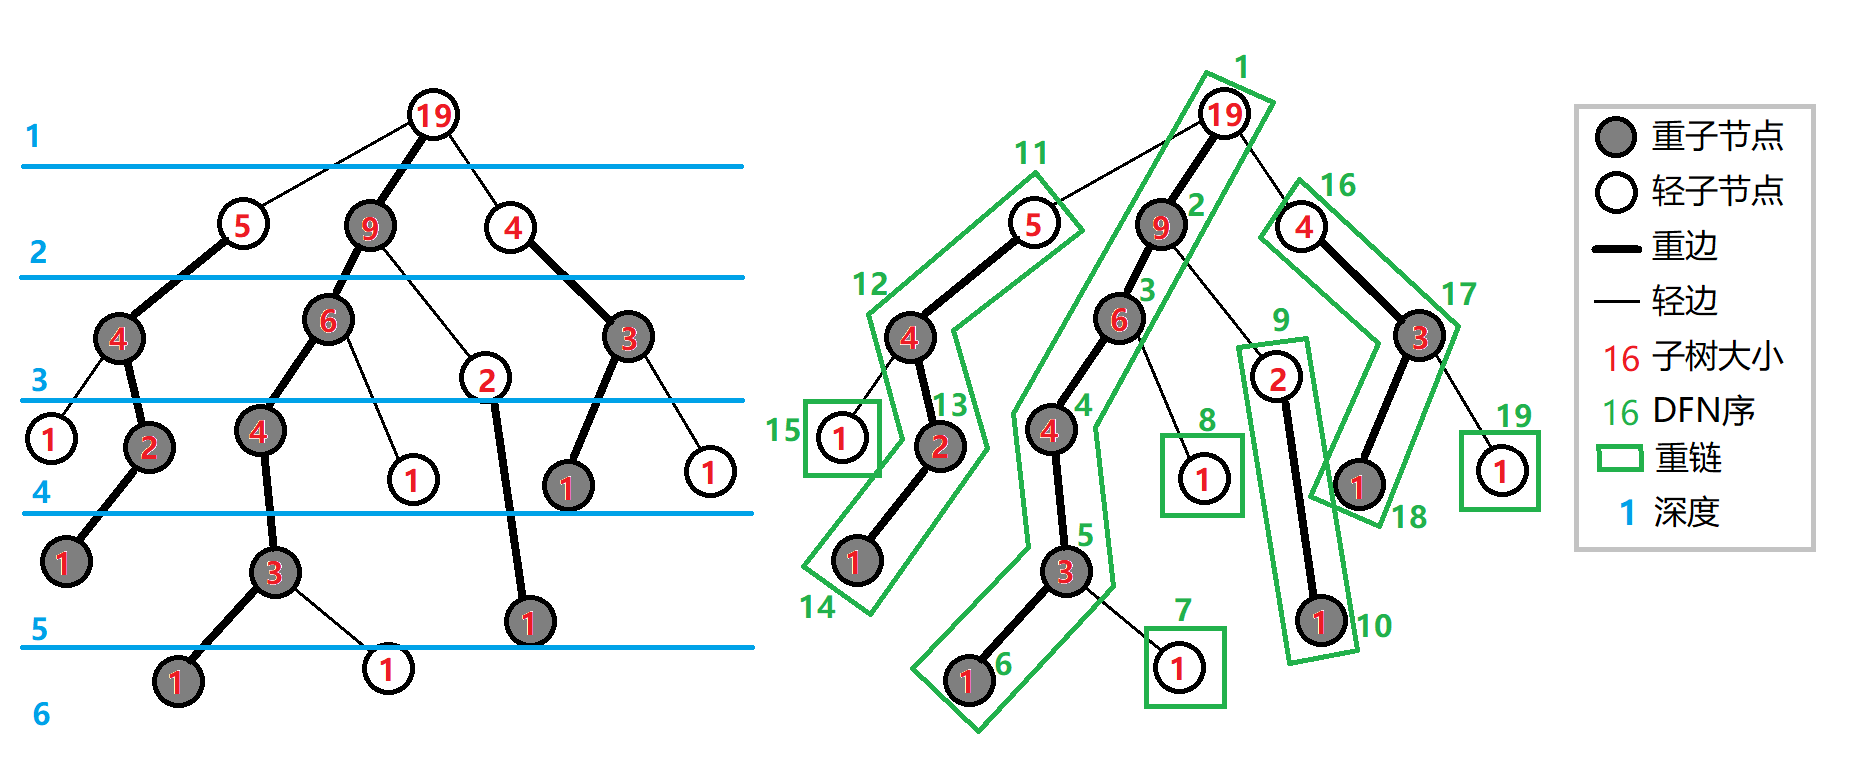
\includegraphics[width=10cm]{picture/图论/树/1.png}
		\caption{重链剖分图例}
	\end{figure}\par
	不难发现,每个轻子节点都是链顶,且每条链都是一个轻子节点后面跟着一大坨的重子节点。
	
	\subsubsection{实现}
	重链剖分的实现分为了两个 dfs 的过程。\par
	对于第一个 dfs,需要记录每个点的父节点,深度,子树大小,重子节点。
	\begin{lstlisting}
const int MAXN = 1e5+5;
int dep[MAXN],siz[MAXN],fa[MAXN],hson[MAXN];
//siz 是子树大小;hson 是重子节点
void dfs1(int u, int d)
{
	siz[u] = 1;		//千万别忘了把 size 初始赋为 1
	dep[u] = d;
	for(int i = e[u].size()-1;i >= 0;i--)
	{
		int v = e[u][i];
		if(v == fa[u]) continue;
		fa[v] = u;
		dfs1(v, d+1);
		if(siz[v] > siz[hson[u]]) hson[u] = v;	//取 size 最大的为重子节点
		siz[u] += siz[v];
	}
}
	\end{lstlisting}\par
	第二个 dfs 记录每个点所在链的链顶(一般来说要初始化为该点本身)、dfn,即 dfs 序、rnk,即 dfs 序对应的编号。\par
	dfs 时,要求优先遍历重子节点。这样就可以保证一条链上的 dfn 是连续的。
	\begin{lstlisting}
const int MAXN = 1e5+5;
int top[MAXN],dfn[MAXN],rnk[MAXN],dfncnt;
void dfs2(int u, int t)
{
	top[u] = t; //记录链顶
	dfn[u] = ++dfncnt; //记录 dfn 序
	rnk[dfncnt] = u;
	if(hson[u]) dfs2(hson[u], t); //先遍历重子节点,注意一定要判断是否有重子节点
	for(int i = e[u].size()-1;i >= 0;i--)
	{
		int v = e[u][i];
		if(v == hson[u] || v == fa[u]) continue;
		//到这里 v 一定是轻子节点
		dfs2(v, v); //上面说过了,轻子节点一定是链顶,应此第二个参数填 v
	}
}
	\end{lstlisting}\par
	重链剖分的变量还是挺多的,有时候还会忘记操作。因此可以先把数组都打好,然后对着有的数组来检查操作是否都做完了。亲测好用。
	\subsubsection{重链剖分性质}
	树上每个节点都属于且仅属于一条重链。\par
	
	
	
	\chapter{连通性相关}
	\section{相关定义与前置知识}
	无向图的连通性主要研究割点和割边。
	\begin{itemize}
		\item 割点:在无向图中,删去该点后会使连通分量数增加的点为 \texttt{割点}。
		\item 割边:在无向图中,删去该边后会使连通分量数增加的边为 \texttt{割边},也称作 \texttt{桥}。
	\end{itemize}
	\noindent
	孤立点和孤立边上的端点都不是给点,但孤立边是割边(这其实是显然的)。\par
	显然,割点和割边重要的原因就是删去他们后相较于非割点和非割边对图的连通性有更大的影响。下面还有几个概念,都是基于刚才的割点和割边的。\par
	\begin{itemize}
		\item 点双连通图:不存在割点的无向连通图被称为 \texttt{点双连通图}。孤立点和孤立边均为点双连通图。
		\item 边双连通图:不存在割边的无向连通图被称为 \texttt{边双连通图}。孤立点是边双连通图,孤立边不是。
		\item 点双连通分量:一张图的极大点双连通子图称为 \texttt{点双连通分量(V-BCC)},简称 \texttt{点双}。
		\item 边双连通分量:一张图的极大边双连通子图称为 \texttt{边双连通分量(E-BCC)},简称 \texttt{边双}。
	\end{itemize}
	
	在连通性这一块,我们用的均为 Tarjan 算法。因此,还需要知道 \texttt{DFS 生成树}。\par
	有向图的 DFS 生成树主要有 4 种边(不一定全部出现):
	\begin{itemize}
		\item 树边(tree edge):绿色边,每次搜索找到一个还没有访问过的结点时就形成了一条树边。
		\item 返祖边(back edge):黄色边,即指向祖先结点的边(Tarjan 中用栈来判断)。
		\item 横插边(cross edge):红色边,在搜索过程中访问过且不在栈中的结点的边。
		\item 前向边(forward edge):蓝色边,搜索中遇到子树中的结点的边。
	\end{itemize}
	对于无向图,不存在横插边和前向边。
	\begin{figure}[H]
		\centering
		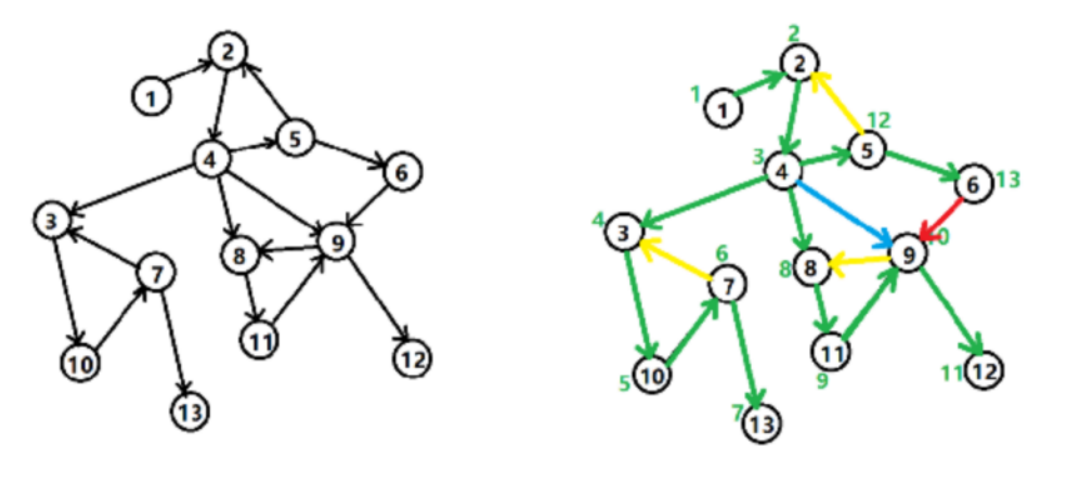
\includegraphics[width=10cm]{picture/图论/连通性相关/1.png}
		\caption{DFS 生成树图例}
	\end{figure}
	其实说实话这些东西知道了也没啥用。
	
	
	\section{割点}
	\subsection{过程}
	不难想到可以尝试删除一个点,然后判断此图的连通性。但这样做复杂度会极高。应此我们需要用到 tarjan 算法。\par
	设点 $x\in V$ 的子树为 $x$ 在 DFS 树上的子树,包含 $x$ 本身,记其为 $T(x)$。记 $\complement_{V}T(x) = T^{\prime}(x)$。
	\subsubsection{对于非根节点的判定:}
	设 $x$ 不为 DFS 生成树的根,则 $T^{\prime}(x) \not= \varnothing$。\par
	若 $x$ 为割点,则删去后,对于 $z \in T^\prime(x)$, 存在 $y$ 使 $y,z$ 不连通,而删除 $x$ 后,所有 $T^\prime(x)$ 的边均存在,则 $y\in T(x)$。如果 $y$ 与 $z$ 不连通,因为 $T^\prime(x)$ 的连通性不变,既均连通,则 $y$ 与所有 $T^\prime(x)$ 中的点都不连通。\par
	推出:若存在 $ y \in T(x)$ 在不经过 $x$ 的情况下与 $T^\prime(x)$ 中所有点均不连通,则 $x$ 就是割点。\par
	现在我们思考怎么判断对于一个 $y \in T(x)$,是否在不经过 $x$ 的情况下与 $T^\prime(x)$ 中所有点都不连通。\par
	注意到,如果 $y\in T(x)$ 不经过 $x$ 就和 $T^\prime(x)$ 连通,就一定存在从 $y$ 到 $T^\prime(x)$ 的一条路径。我们称这条路径在 $T^\prime(x)$ 的第一个结点为 $v$,倒数第二个,也就是最后一个在 $T(x)$ 上的结点为 $u$。如果 $(u,v)$ 是树边,那么 $u=x$,矛盾。则 $v$ 应该是 $u$ 的祖先。又因为 $x$ 是 $u$ 的祖先,$v\in T^\prime(x)$,则 $v$ 也是 $x$ 的祖先。\par 
	这时我们发现,$x$ 不是割点,那么就会有一条\texttt{非树边}使 $y\in T(x)$ 连向 $x$ 的祖先。这个可以用时间戳来判断。设 $f_x$ 表示与 $x$ 通过\texttt{非树边}相连的点的时间戳的最小值,则可写为 $f_x < dfn_x$。\par
	因为 $x$ 的不同儿子子树之间没有非树边(子树独立性),设 $x$ 的儿子 $y^\prime$ 的子树包含 $y$,即 $y\in T(y^\prime)$。\par
	\begin{itemize}
		\item 对于 $T(y^\prime)$,如果存在 $u\in T(y^\prime)$ 满足 $f_u < dfn_u$,那么删除 $x$ 后 $T(y^\prime)$ 的每个点与 $T^\prime(x)$ 均连通。这时 $u$ 与 $T^\prime(x)$ 中的某个点通过非树边直接连通,$T(y^\prime)$ 中的所有点均通过树边连通。此时 $x$ 不是割点。\par
		\item 反之,如果不存在 $u\in T(y^\prime)$ 满足 $f_u < dfn_u$,那么删除 $x$ 后 $T(y^\prime)$ 的每个点与 $T^\prime(x)$ 均不连通。此时 $x$ 是割点。且只需要出现一个 $y^\prime$ 满足这个条件就可以判断出 $x$ 是割点。
	\end{itemize}\par
	原本我们需要判断 $T(x)$ 上的所有点去检查 $f_u < dfn_u$ 的情况是否出现。现在令 $low_x$ 表示与 $x$ 及其子树上的所有点通过非树边相连接的点的时间戳的最小值,则可以只通过 $low_x$ 判断即可。
	这样我们就得到了在 $x$ 为非根节点情况下的割点判定方法:\par
	
	{
		\kaishu
		对于一个非根节点 $x$,$x$ 是割点当且仅当存在 $y$ 是 $x$ 的子节点,有 $low_y \geq dfn_x$。
	}
	\subsubsection{对于根节点的判定:}
	根节点的判定相对简单。\par
	设点 $x$ 是 DFS 树上的根节点。\par
	若 $x$ 有大于一个子节点,根据子树独立性,删去 $x$ 后其子节点的子树各不相通,所以 $x$ 是割点。反之,若 $x$ 有小于等于一个子节点,删去后剩余部分通过树边连通,$x$ 不是割点。\par
	\par
	这样我们就得到了判断割点的完整方法。
	
	\subsection{实现}
	\subsubsection{解释}
	$dfn$:某个点被遍历到的时间戳。\par
	$low$:某个点通过非树边到达最早的点的时间戳。\par
	$is\_cut$:是否为割点。\par
	$cutcnt$:统计割点个数。\par
	在 dfs 过程中求出 dfn 和 low,然后进行对割点的判断。
	\subsubsection{代码}
	\noindent
	此代码用 vector 存图。
	\begin{lstlisting}
vector<int> e[MAXN];
int dfn[MAXN];
int low[MAXN];
int cnt;
bool is_cut[MAXN];
int cutcnt;

void tarjan(int u,int f,int root)
{
	dfn[u] = low[u] = ++cnt;
	int son = 0; //用于统计子节点个数
	for(int i = e[u].size()-1;i >= 0;i--)
	{
		int v = e[u][i];
		if(v == f) continue;
		if(!dfn[v])//说明这个 v 是在 x 的子树中的
		{
			son++;
			tarjan(v,u,root);
			low[u] = min(low[u],low[v]);
			if(dfn[u] <= low[v])
			{
				if(!is_cut[u] && u != root)
				{
					//非根节点的情况
					cutcnt++;
					is_cut[u] = true;
				}
			}
		}
		else low[u] = min(low[u],dfn[v]);
		//这个 else 中 v 不再 x 的子树当中。
		//而我们求的是 x 子树当中 low 的最小值。
		//因此 min 的第二个参数是 dfn[v] 而不是 low[v]。
	}
	if(u == root && son >= 2) is_cut[root] = true,cutcnt++;
	//根节点的情况
}
	\end{lstlisting}
	
	\section{割边}
	\subsection{过程}
	和割点差不多。\par
	树边能使整张图连通,因此割掉非树边后不影响连通性。因此 $e=(u,v)$ 是割边的必要条件是 $e$ 为树边。\par
	不妨设 $v$ 是 $u$ 的儿子。若割掉 e 后图不连通,根据求割点的经验,不难发现当 $low_v > dfn_u$ 时,$e$ 为割边。
	\subsection{实现}
	还没写...
	\section{点双连通分量}
	\subsection{实现}
	\section{边双连通分量}
	\subsection{实现}
	\section{强连通分量}
	\subsection{实现}
	\subsubsection{解释}
	$sta$:栈。\par
	$top$:栈顶。\par
	$insta$:判断是否在栈中。\par
	$belong$:判断点 $i$ 在哪个强连通分量中。
	\subsubsection{代码}
	\noindent
	此代码用 vector 存图。
	\begin{lstlisting}
vector<int> e[MAXN];
int low[MAXN],dfn[MAXN],dfncnt,belong[MAXN],sc;
int sta[MAXN],top;bool insta[MAXN];
void tarjan(int u)
{
	low[u] = dfn[u] = ++dfncnt;
	sta[++top] = u,insta[u] = true;
	for(int i = e[u].size()-1;i >= 0;i--)
	{
		int v = e[u][i];
		if(!dfn[v])
		{
			tarjan(v);
			low[u] = min(low[u],low[v]);
		}
		else if(insta[v])
		{
			low[u] = min(low[u],low[v]);
		}
	}
	
	if(dfn[u] == low[u])
	{
		sc++;int now;
		do
		{
			now = sta[top];
			insta[now] = false;
			belong[now] = sc;
			sz[sc]++;
		} while (sta[top--]!=u);
	}
}
	\end{lstlisting}
	
	
\end{document}